% The section about testing the basic workings of the software
% @author Kalvin Döge
%


\section{Überprüfen der Grundfunktionalität}\label{sec:testing}

Um die Funktionalität des Modells zu bestätigen, sind die folgenden Kernelemente im Quelltext überprüft:

\textbf{Einbindung und Verifikation aller \code{TrafficLight}s:} Zur Verifikation, ob alle 1260 \code{TrafficLight}s aus der GeoJSON von OpenStreetMap~\cite{OSF2004} richtig exportiert sind, werden die extrahierten Daten in die Online-Anwendung ,,kepler.gl``~\cite{Kepler2018} eingegeben, die die \code{Longitude-Latitude}-Daten der GeoJSON auf einer virtuellen Weltkarte darstellt:

\begin{figure}[h]
    \centering
    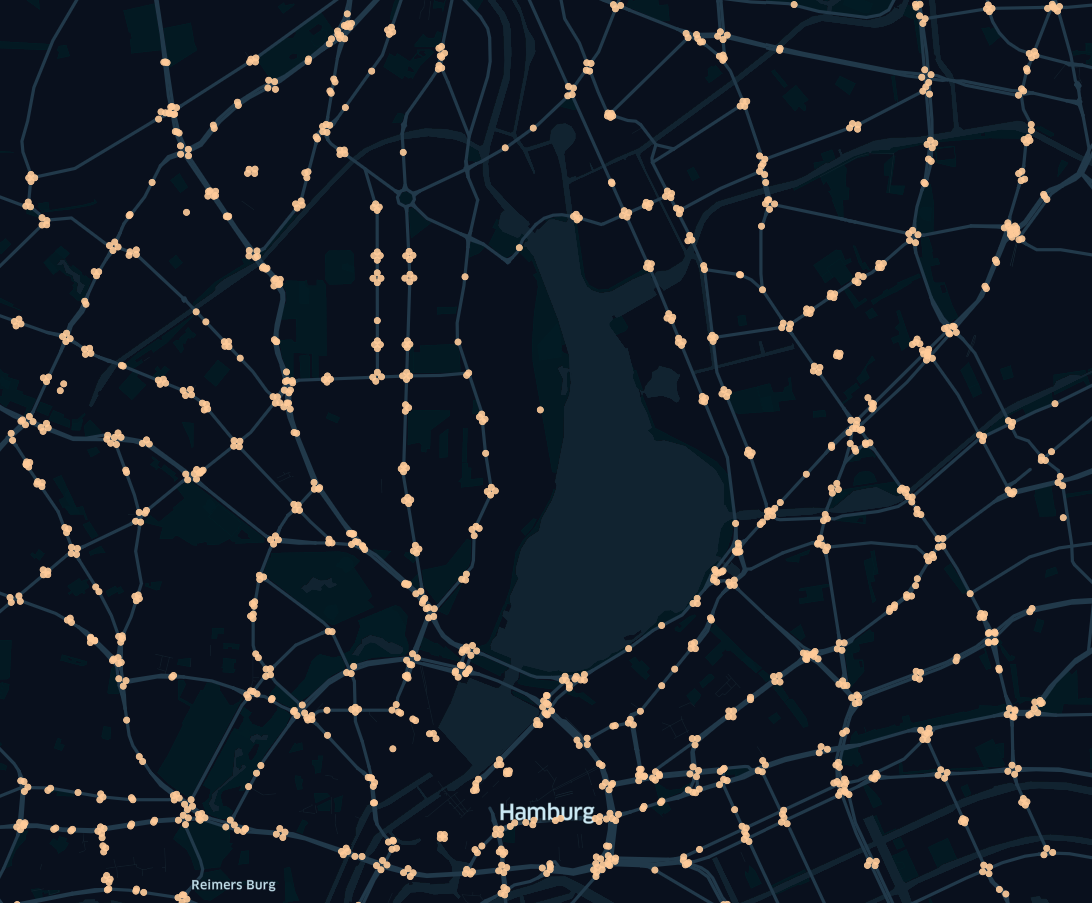
\includegraphics[width=0.50\textwidth]{testing-trafficlightlayer}~\caption{Der Export von OpenStreetMap in kepler.gl eingefügt}
    \label{fig:traffic-light-spawns}
\end{figure}

Die Verteilung der Lichtsignalanlagen auf Kreuzungen und Straßen, wie man sie in der Abbildung~\ref{fig:traffic-light-spawns} sehen kann, entspricht der Position in OpenStreetMap, wie man anhand des Vergleichs in~\ref{fig:traffic-light-spawns-comparison} erkennen kann.

\begin{figure}[h]
    \centering
    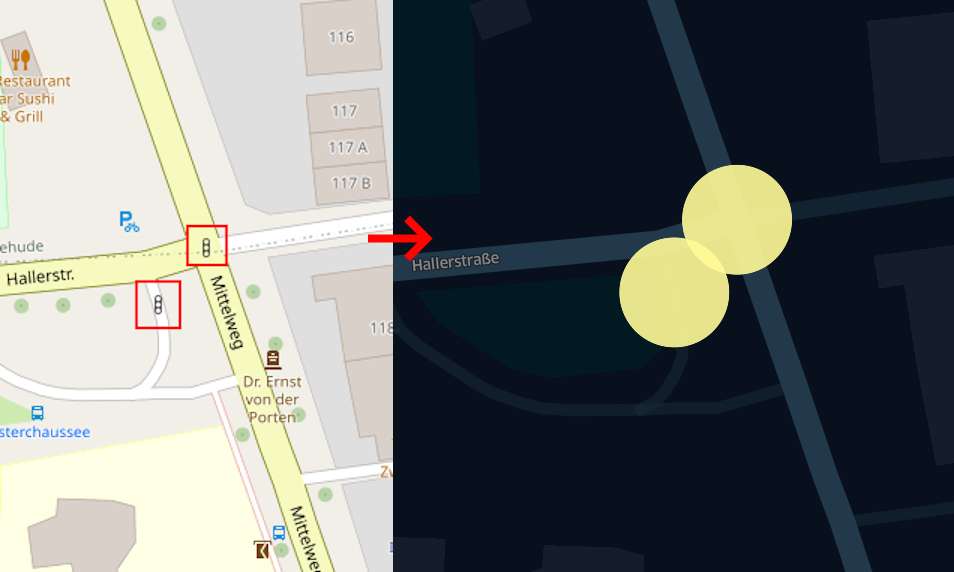
\includegraphics[width=0.75\textwidth]{testing-trafficlightlayer-comparison}~\caption{Lichtsignalanlagen an der Kreuzung der Hallerstraße, links in OpenStreetMap, rechts in kepler.gl eingefügt}
    \label{fig:traffic-light-spawns-comparison}
\end{figure}

Zur Überprüfung, ob bei der Initialisierung des \code{TrafficLightLayer}s alle Lichtsignalanlagen richtig importiert wurden, ist nach dem Einbinden über die \code{InitLayer()}-Methode eine Abfrage auf die Anzahl der eingelesenen \code{TrafficLight}s eingebaut, wie in der Abbildung~\ref{fig:all-traffic-lights} zu sehen ist:

\begin{figure}[h]
    \centering
    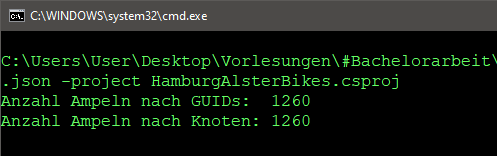
\includegraphics[width=0.75\textwidth]{testing-trafficlightlayer-all}~\caption{Die Konsolenausgabe der aktuell eingebauten \code{TrafficLight}s}
    \label{fig:all-traffic-lights}
\end{figure}

Die Überprüfung, ob die GeoJSON in OpenStreetMap korrekt und vollständig ist im Vergleich zur Realität, lässt sich nur mit einem großen Aufwand überprüfen.
Dafür müsste man bei jeder Schaltung selbst physisch vor Ort sein und die Position bestätigen.
Dahingehend wird die Ausgabe von OpenStreetMap so hingenommen und als ausreichend für diese Simulation festgelegt.

\textbf{Einbindung und Verifikation der \code{HumanTraveler} und {BicycleLeader}:}

Zur Überprüfung, ob die \code{HumanTraveler} und \code{BicycleLeader} korrekt in der Simulation erschaffen werden, wird erneut über kepler.gl die ausgegebenen GeoJSON überprüft:

\begin{figure}[h]
    \centering
    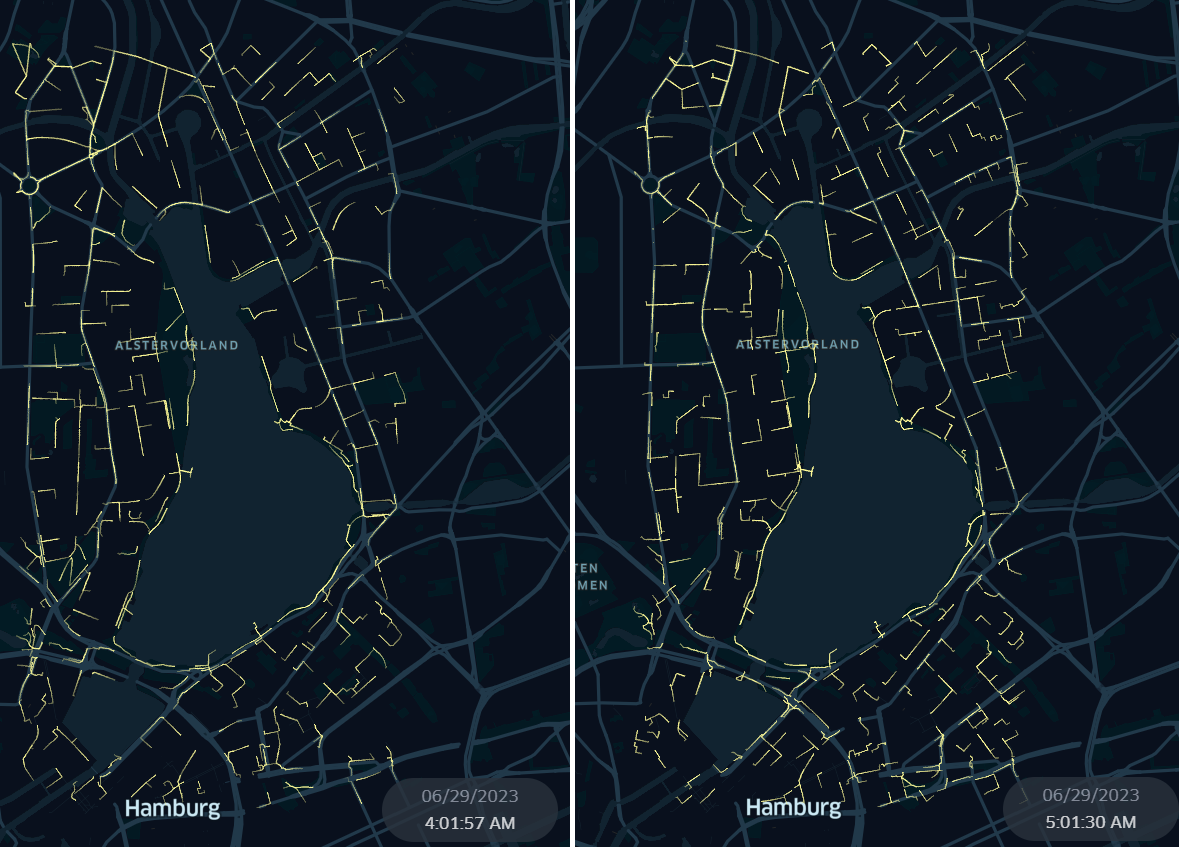
\includegraphics[width=0.75\textwidth]{testing-humantraveler-creation}~\caption{Der Erstellbereich der \code{HumanTraveler}, links von 4 Uhr und rechts von 5 Uhr morgens}
    \label{fig:spawning-human-traveler}
\end{figure}

\begin{figure}[h]
    \centering
    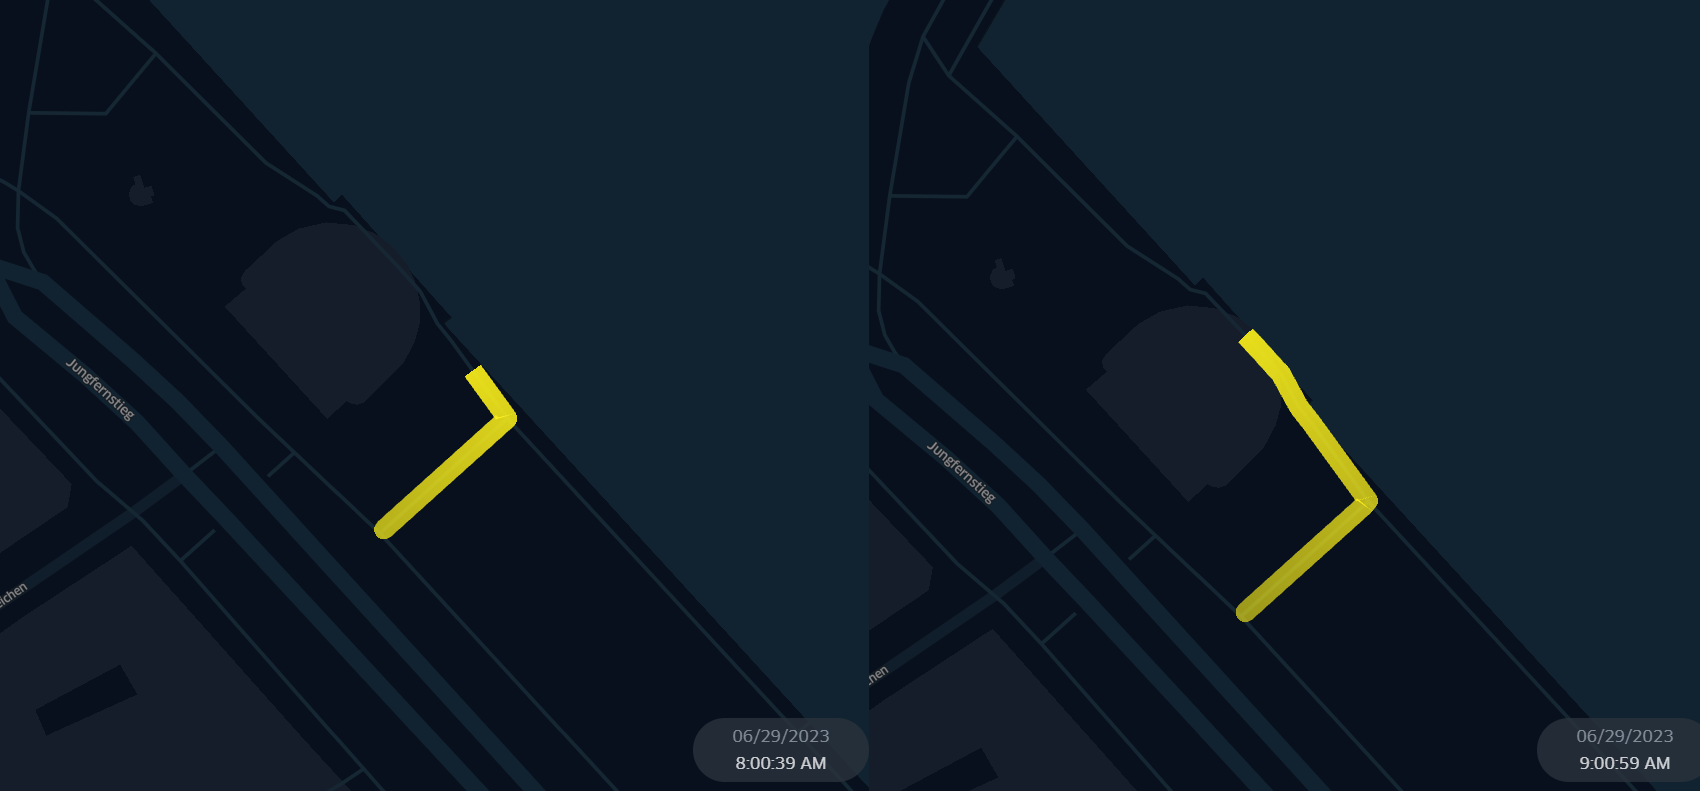
\includegraphics[width=0.5\textwidth]{testing-bicycleleader-creation}~\caption{Die Erschaffung des \code{BicycleLeader}, links um 8 Uhr, rechts um 9 uhr morgens}
    \label{fig:spawning-bicycle-leader}
\end{figure}

Aus der Grafik von~\ref{fig:spawning-human-traveler} und~\ref{fig:spawning-bicycle-leader} lässt sich erkennen, dass die stündliche Erschaffung korrekt funktioniert.
Einerseits ist der Simulationsbereich erkennbar, die rechteckige Form, die von den Pfaden der \code{HumanTraveler} erzeugt wird, als auch ihr Auftreten überhaupt.

Ebenfalls ist die korrekte Interaktion mit den \code{TrafficLight}s zu überprüfen.
\code{HumanTraveler} und \code{BicycleLeader} verwenden die Funktion \code{IsWaitingAtTrafficLight()}, die die Agenten bei Ankunft an einer Lichtsignalanlage zur Warteschlange hinzufügt.
Wie aus dem Konsolenausschnitt von~\ref{fig:waiting-at-traffic-light-humantraveler} zu entnehmen ist, können die Agenten korrekt mit den \code{TrafficLight}s interagieren.

\begin{figure}[h]
    \centering
    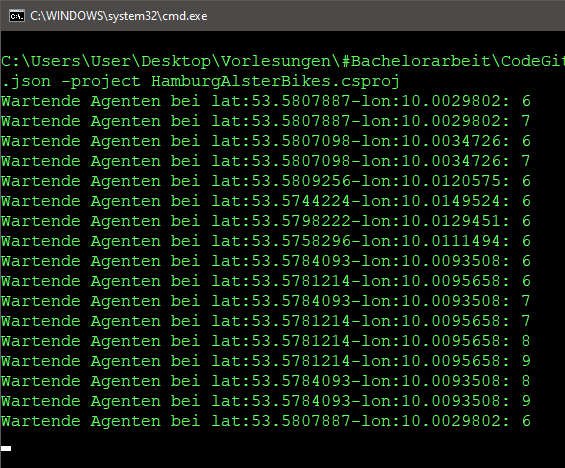
\includegraphics[width=0.5\textwidth]{testing-humantraveler-waiting}~\caption{Hier wird eine Ausgabe an Lichtsignalanlagen gegeben, sobald mehr als 5 Agenten in der Warteschlange einer \code{TrafficLight} sind.}
    \label{fig:waiting-at-traffic-light-humantraveler}
\end{figure}

Die Konsolenausgabe~\ref{fig:waiting-at-traffic-light-humantraveler} sind alle von den \code{HumanTravelers}, da ein Anhalten der \code{BicycleLeader} separat überprüft wird und dann zur Entfernung aus der Simulation führt, wie in der folgenden Konsolenausgabe~\ref{fig:waiting-at-traffic-light-bicycleleader} erkennbar ist.

\begin{figure}[h]
    \centering
    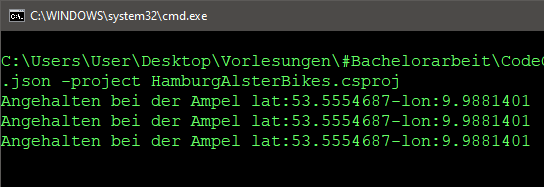
\includegraphics[width=0.75\textwidth]{testing-bicycleleader-stop}~\caption{Konsolenausgabe, bei der \code{BicycleLeader} alle 3 Stunden in Folge wegen der zu langen Rot-Signalphase die Abbruchbedingung erreicht.}
    \label{fig:waiting-at-traffic-light-bicycleleader}
\end{figure}

Hat der \code{BicycleLeader} erfolgreich den letzten Punkt erreicht, so wird dann nur noch geprüft, ob der letzte Punkt der zu fahrenden Route identisch zu der aktuellen Position des Agenten ist.
Dies wird bewerkstelligt, wie man in der Konsolenausgabe aus~\ref{fig:testing-successful-trip} indem die Distanz zwischen den beiden Punkten 0 sein muss.

\begin{figure}[h]
    \centering
    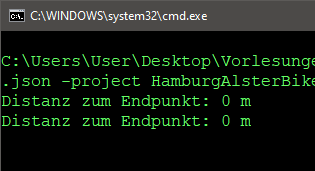
\includegraphics[width=0.75\textwidth]{testing-distance}~\caption{Distanzangabe über die Konsole vom letzten, zu erreichenden Punkt, bis zum \code{BicycleLeader}.}
    \label{fig:testing-successful-trip}
\end{figure}


Zuletzt wird noch geprüft, ob die \code{HumanTraveler} anhalten, sobald sie in die Warteschlange einer \code{TrafficLight} hinzugefügt werden.
Dafür wird, wie in der Konsolenausgabe~\ref{fig:human-traveler-slowing-down} sichtbar, die Geschwindigkeit nach einer Wartezeit von 5 Sekunden beziehungsweise 5 Ticks ausgegeben, um dem \code{HumanTraveler} Zeit zu geben, die Bremsen zu aktivieren und zu entschleunigen.

\begin{figure}[h]
    \centering
    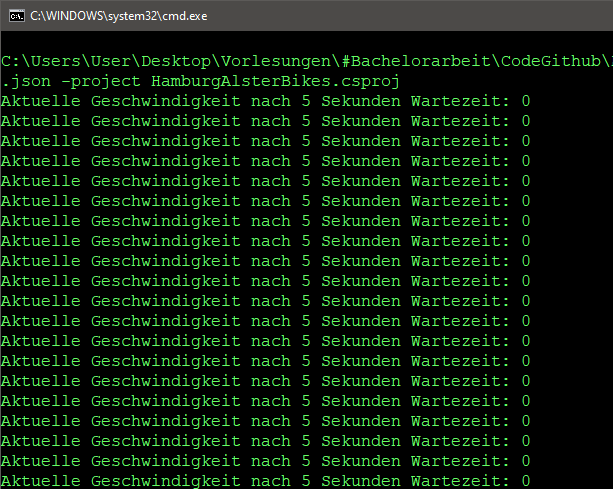
\includegraphics[width=0.5\textwidth]{testing-velocity-after-stopping}~\caption{Konsolenausgabe, bei der \code{HumantTraveler} nach 5 Sekunden warten an einer \code{TrafficLight} ihre Geschwindigkeit ausgeben.}
    \label{fig:human-traveler-slowing-down}
\end{figure}
